\documentclass[english]{beamer}\usepackage[]{graphicx}\usepackage[]{color}
%% maxwidth is the original width if it is less than linewidth
%% otherwise use linewidth (to make sure the graphics do not exceed the margin)
\makeatletter
\def\maxwidth{ %
  \ifdim\Gin@nat@width>\linewidth
    \linewidth
  \else
    \Gin@nat@width
  \fi
}
\makeatother

\definecolor{fgcolor}{rgb}{0.345, 0.345, 0.345}
\newcommand{\hlnum}[1]{\textcolor[rgb]{0.686,0.059,0.569}{#1}}%
\newcommand{\hlstr}[1]{\textcolor[rgb]{0.192,0.494,0.8}{#1}}%
\newcommand{\hlcom}[1]{\textcolor[rgb]{0.678,0.584,0.686}{\textit{#1}}}%
\newcommand{\hlopt}[1]{\textcolor[rgb]{0,0,0}{#1}}%
\newcommand{\hlstd}[1]{\textcolor[rgb]{0.345,0.345,0.345}{#1}}%
\newcommand{\hlkwa}[1]{\textcolor[rgb]{0.161,0.373,0.58}{\textbf{#1}}}%
\newcommand{\hlkwb}[1]{\textcolor[rgb]{0.69,0.353,0.396}{#1}}%
\newcommand{\hlkwc}[1]{\textcolor[rgb]{0.333,0.667,0.333}{#1}}%
\newcommand{\hlkwd}[1]{\textcolor[rgb]{0.737,0.353,0.396}{\textbf{#1}}}%
\let\hlipl\hlkwb

\usepackage{framed}
\makeatletter
\newenvironment{kframe}{%
 \def\at@end@of@kframe{}%
 \ifinner\ifhmode%
  \def\at@end@of@kframe{\end{minipage}}%
  \begin{minipage}{\columnwidth}%
 \fi\fi%
 \def\FrameCommand##1{\hskip\@totalleftmargin \hskip-\fboxsep
 \colorbox{shadecolor}{##1}\hskip-\fboxsep
     % There is no \\@totalrightmargin, so:
     \hskip-\linewidth \hskip-\@totalleftmargin \hskip\columnwidth}%
 \MakeFramed {\advance\hsize-\width
   \@totalleftmargin\z@ \linewidth\hsize
   \@setminipage}}%
 {\par\unskip\endMakeFramed%
 \at@end@of@kframe}
\makeatother

\definecolor{shadecolor}{rgb}{.97, .97, .97}
\definecolor{messagecolor}{rgb}{0, 0, 0}
\definecolor{warningcolor}{rgb}{1, 0, 1}
\definecolor{errorcolor}{rgb}{1, 0, 0}
\newenvironment{knitrout}{}{} % an empty environment to be redefined in TeX

\usepackage{alltt}
%% The most common packages are already included in:
\usetheme{biostat}
%%%%%%%%%%%%%%%%%%%%%%%%%%%%%%%%%%%%%%%%%%%%%%%%%%%%%%%% 
\usepackage{amsmath,amsfonts,tikz, amssymb}
\usetikzlibrary{trees}

%% Header data: (adjust to your needs:
\def\uzhunit{Biostatistics}             %% if (not) needed comment/uncomment
%\def\uzhunitext{STA480}

\title{Publication Bias in Meta-Analysis}%[Publication Bias]
%% Optional Argument in [Brackets]: Short Title for Footline

%% The following are all optional, simply comment them
%\subtitle{Publication Bias in the Cochrane Libary}
%\institute{Biostatistics Journal Club}  %% optional
\author{Giuachin Kreiliger}
%\date{\today}
%%%%%%%%%%%%%%%%%%%%%%%%%%%%%%%%%%%%%%%%%%%%%%%%%%%%%%%% 




%%%%%%%%%%%%%%%%%%%%%%%%%%%%%%%%%%%%%%%%%%%%%%%%%%%%%%%%
\IfFileExists{upquote.sty}{\usepackage{upquote}}{}
\begin{document}
\maketitle
%%%%%%%%%%%%%%%%%%%%%%%%%%%%%%%%%%%%%%%%%%%%%%%%%%%%%%%% 

\begin{frame}{Cochrane Library}
Database of high-quality, systematic reviews in clinical science.

Currently $\sim$ 8,000 reviews, prepared by independent groups. 

Reviews are peer-reviewed and prepared after guidelines.
\end{frame}


\begin{frame}{Cochrane Library Dataset}
5,016 systematic reviews with studies published until 2018.

52,995 studies.

463,820 study results.
\end{frame}


\begin{frame}{Dataset Structure}

\begin{figure}
\tikzstyle{every node}=[draw=black,thick,anchor=west,scale=.65]
\tikzstyle{selected}=[draw=red,fill=red!30]
\tikzstyle{optional}=[dashed,fill=gray!50]
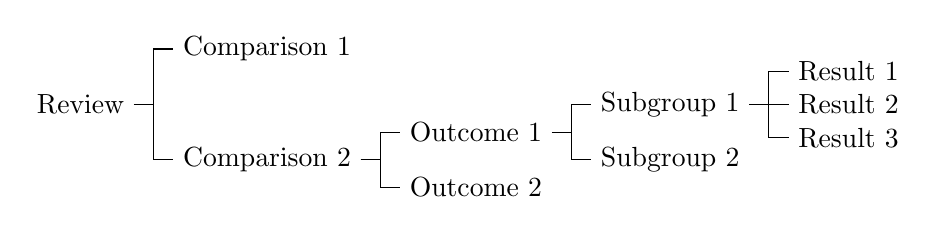
\begin{tikzpicture}
[grow = right, anchor = west,
  growth parent anchor=east, % added code
  parent anchor=east, level distance=.5cm,
  sibling distance=2em, level 1/.style={sibling distance=2em}, level 2/.style={sibling distance=2em},
  level 3/.style={sibling distance=2em}, level 4/.style={sibling distance=1.2em}]
  \node {Review} [edge from parent fork right]
    child { node {Comparison 2}
      child { node {Outcome 2}}
      child { node {Outcome 1}
        child { node {Subgroup 2}}
        child { node {Subgroup 1}
          child  { node {Result 3}}
          child  { node {Result 2}}
          child  { node {Result 1}}
          }}
    }
    child [missing] {}
    child { node {Comparison 1}};
\end{tikzpicture}
%\caption{Structure of a hypothetical review with two different comparisons\label{review.structure}}
\label{review.structure}
\end{figure}
\end{frame}


\begin{frame}{Dataset Structure}
\begin{itemize}
\item Comparison: What is compared, e.g. treatment vs. control
\item Outcome: How it is compared
\item Subgroup: Subgroup affiliation
\item Meta-Analysis Group: Results from same comparison, outcome and subgroup
\end{itemize}
\end{frame}


\begin{frame}[fragile]{Review Example: binary outcome}
Barbiturate efficacy for head injury treatment
\vspace{-5mm}
% latex table generated in R 3.5.1 by xtable 1.8-3 package
% Tue May 14 15:03:41 2019
\begin{table}[ht]
\centering
\begingroup\tiny
\begin{tabular}{lllrrrr}
  \hline
Study & Comparison & Outcome & Events & Total & Events\_c & Total\_c \\ 
  \hline
Bohn 1989 & Barbiturate vs no b & Death at the end of & 11 & 41 & 11 & 41 \\ 
  Bohn 1989 & Barbiturate vs no b & Death or severe dis & 18 & 41 & 13 & 41 \\ 
  Eisenberg 1988 & Barbiturate vs no b & Uncontrolled ICP du & 25 & 37 & 30 & 36 \\ 
  Eisenberg 1988 & Barbiturate vs no b & Hypotension during  & 23 & 37 & 18 & 36 \\ 
  Perez-Barcena 2008 & Pentobarbital vs Th & Death at the end of & 16 & 21 & 9 & 21 \\ 
  Perez-Barcena 2008 & Pentobarbital vs Th & Death or severe dis & 17 & 21 & 13 & 21 \\ 
  Perez-Barcena 2008 & Pentobarbital vs Th & Uncontrolled ICP du & 18 & 22 & 11 & 22 \\ 
  Perez-Barcena 2008 & Pentobarbital vs Th & Hypotension during  & 20 & 22 & 21 & 22 \\ 
  Schwartz 1984 & Barbiturate vs Mann & Death at the end of & 6 & 15 & 7 & 14 \\ 
  Schwartz 1984 & Barbiturate vs Mann & Uncontrolled ICP du & 19 & 28 & 12 & 31 \\ 
  Ward 1985 & Barbiturate vs no b & Mean ICP during tre & 0 & 27 & 0 & 26 \\ 
  Ward 1985 & Barbiturate vs no b & Mean arterial press & 0 & 27 & 0 & 26 \\ 
  Ward 1985 & Barbiturate vs no b & Mean body temperatu & 0 & 27 & 0 & 26 \\ 
   \hline
\end{tabular}
\endgroup
\label{barbiturates}
\end{table}

\end{frame}


\begin{frame}[fragile]{Dataset Properties}
Missing data:
% latex table generated in R 3.5.1 by xtable 1.8-3 package
% Tue May 14 15:03:41 2019
\begin{table}[ht]
\centering
\begin{tabular}{lr}
  \hline
  \hline
Missing mean values and mean differences & 984 \\ 
  Missing standard deviations and standard errors & 1300 \\ 
  Missing sample sizes & 12173 \\ 
  Missing study year & 44649 \\ 
   \hline
\end{tabular}
\end{table}

\end{frame}


\begin{frame}[fragile]{Dataset Properties}
Review and study properties:
% latex table generated in R 3.5.1 by xtable 1.8-3 package
% Tue May 14 15:03:41 2019
\begin{table}[ht]
\centering
\begingroup\footnotesize
\begin{tabular}{lrrrr}
  & 5\% quantile & median & mean & 95\% quantile \\ 
  \hline
Study number & 1 & 7 & 12 & 40 \\ 
   \hline
\hline
Comparison number & 1 & 2 & 4 & 12 \\ 
  Group number & 2 & 19 & 37 & 132 \\ 
  Study years & 1981 & 2002 & 2000 & 2013 \\ 
   \hline
Study sample size & 13 & 78 & 750 & 890 \\ 
  \end{tabular}
\endgroup
\end{table}

\end{frame}


\begin{frame}[fragile]{Pooling Studies - Meta-Analysis}
Multiple results in a meta-analysis group can be pooled:
% latex table generated in R 3.5.1 by xtable 1.8-3 package
% Tue May 14 15:03:41 2019
\begin{table}[ht]
\centering
\begingroup\footnotesize
\begin{tabular}{rrr}
  \hline
n & Number of groups & Cumulative sum of groups \\ 
  \hline
1 & 102344 & 188079 \\ 
  2 & 31686 & 85735 \\ 
  3 & 16072 & 54049 \\ 
  4 & 9628 & 37977 \\ 
  5 & 6444 & 28349 \\ 
  6 & 4230 & 21905 \\ 
  7 & 2961 & 17675 \\ 
  8 & 2114 & 14714 \\ 
  9 & 1592 & 12600 \\ 
  10 & 11008 & 11008 \\ 
   \hline
\end{tabular}
\endgroup
\label{repr.groups}
\end{table}

\end{frame}

\begin{frame}{Meta-analysis}
Benefits:
\begin{itemize}
\item Summary of evidence (e.g. of a treatment)
\item More reliable evidence (?)
\end{itemize}

Assumptions:
\begin{itemize}
\item Identical study settings (can be relaxed)
\item Random sample of studies
\end{itemize}
\end{frame}


\begin{frame}{Small Study Effects}
``The tendency for the smaller studies to show larger treatment effects'' \citep{Sterne}
\end{frame}


\begin{frame}{Small Study Effects}
Causes:
\begin{itemize}
\item Selective publication of studies with large effects
\item Bias in smaller studies
\item Systematical differences in study settings
\item \ldots
\end{itemize}
\end{frame}


\begin{frame}{Small Study Effect Tests}
Tests applicable if:
\begin{itemize}
\item $n$ large
\item variation in the estimated variances of effects \\(here: $\frac{\sigma_{\textrm{max}}}{\sigma_{\textrm{min}}} > 4$)
\end{itemize}
Adjustments required if variance is dependent on effect size (e.g. log odds ratios)
\end{frame}


\begin{frame}[fragile]{Small Study Effect Tests}
Funnel plots (continuous outcome examples):

\vspace{-1.2cm}

\begin{knitrout}
\definecolor{shadecolor}{rgb}{0.969, 0.969, 0.969}\color{fgcolor}
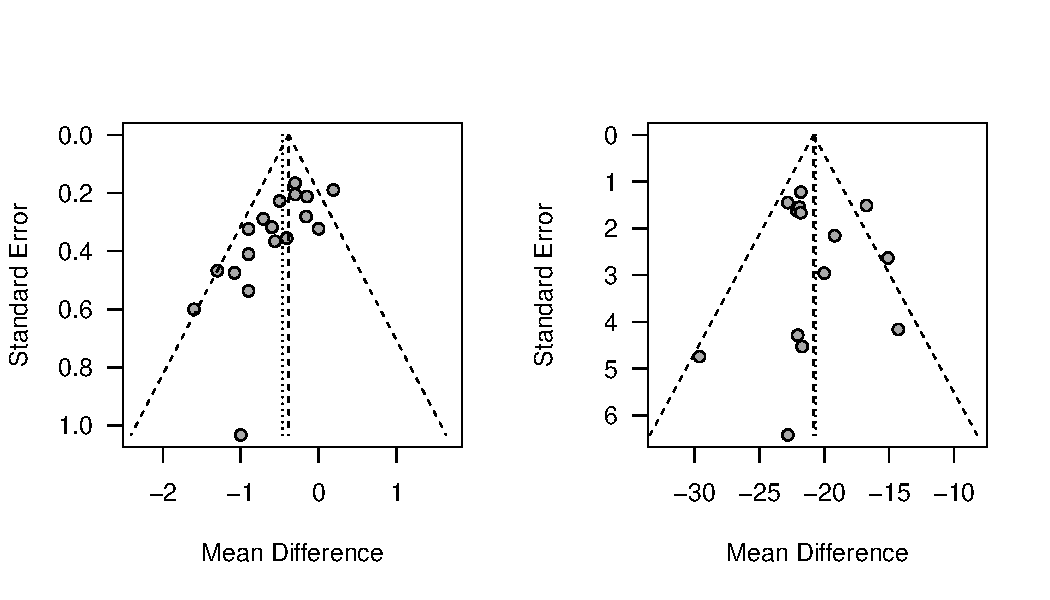
\includegraphics[width=\maxwidth]{figure/unnamed-chunk-6-1} 

\end{knitrout}

\end{frame}


\begin{frame}[fragile]{Regression based Tests}
Radial plots (continuous outcome examples):

\vspace{-1.2cm}

\begin{knitrout}
\definecolor{shadecolor}{rgb}{0.969, 0.969, 0.969}\color{fgcolor}
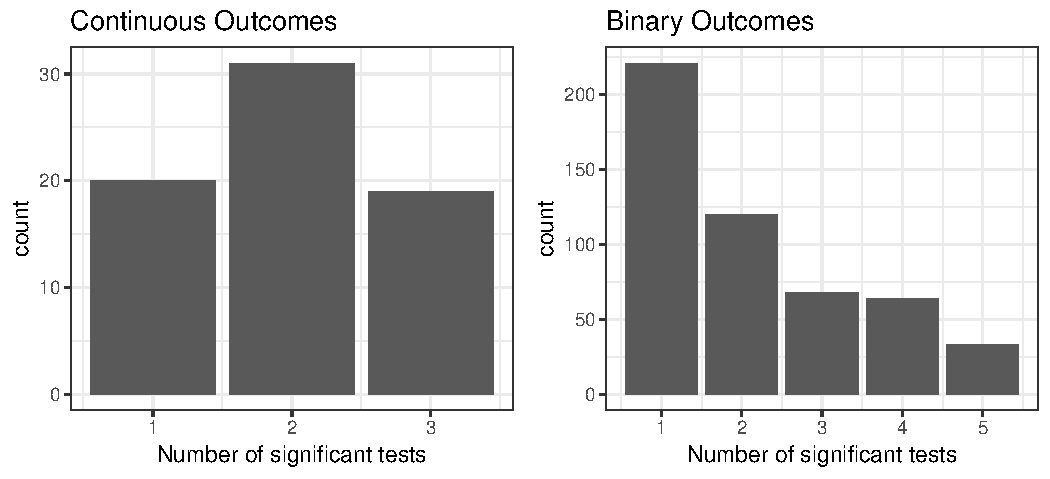
\includegraphics[width=\maxwidth]{figure/unnamed-chunk-7-1} 

\end{knitrout}

\end{frame}


\begin{frame}{Regression based Tests}
Continuous outcomes tests:

$i$ being the $i$th study in a meta-analysis:

Let $y_{i} = \textrm{effect}_{i}/\textrm{se}_{i}$ and $x_{i} = 1/\textrm{se}_{i}$
\begin{itemize}
\item \citet{Egger} : \\ $y_{i} \sim N(\beta_{0} + \beta_{1}x_{i}, v_{i})$
\item \citet{thompson.sharp} : \\ $y_{i} \sim N(\beta_{0} + \beta_{1}x_{i}, v_{i} + \tau^2)$
\end{itemize}
%Test for non-zero intercept $\beta_{0}$
\end{frame}

\begin{frame}[fragile]{Egger's Tests}

\vspace{-6cm}

\begin{knitrout}
\definecolor{shadecolor}{rgb}{0.969, 0.969, 0.969}\color{fgcolor}\begin{kframe}
\begin{verbatim}
## 
## 	Linear regression test of funnel plot asymmetry
## 
## data:  meta.example
## t = -4.095, df = 17, p-value = 0.0007548
## alternative hypothesis: asymmetry in funnel plot
## sample estimates:
##       bias    se.bias      slope 
## -2.4398295  0.5958069  0.2653786
\end{verbatim}
\end{kframe}
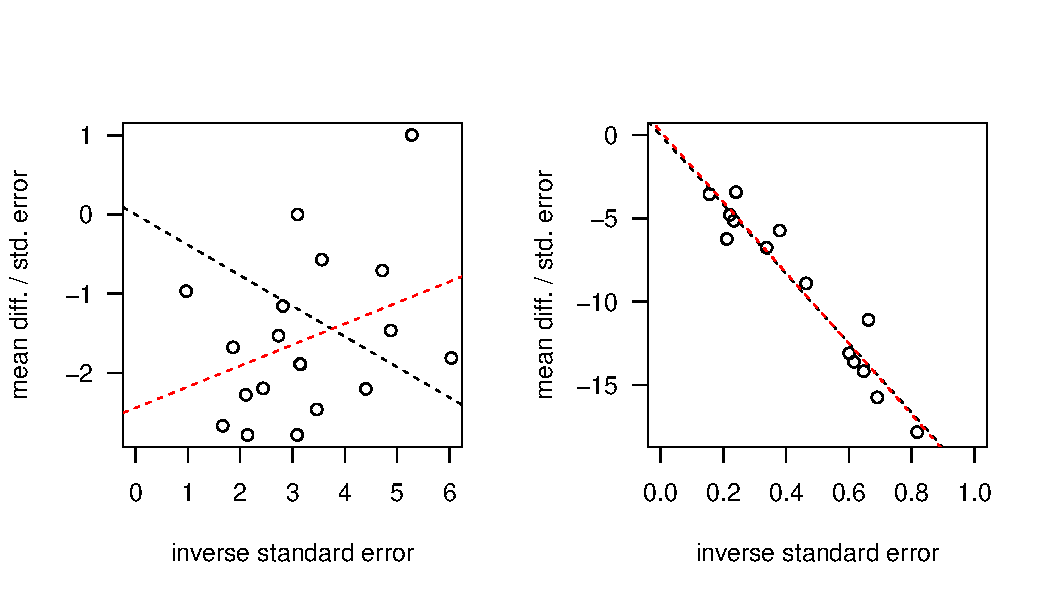
\includegraphics[width=\maxwidth]{figure/unnamed-chunk-8-1} 
\begin{kframe}\begin{verbatim}
## 
## 	Linear regression test of funnel plot asymmetry
## 
## data:  meta.nexample
## t = 0.2718, df = 12, p-value = 0.7904
## alternative hypothesis: asymmetry in funnel plot
## sample estimates:
##        bias     se.bias       slope 
##   0.2324769   0.8553371 -21.2466388
\end{verbatim}
\end{kframe}
\end{knitrout}

\end{frame}


\begin{frame}[fragile]{Thompson and Sharp's Tests}

\vspace{-6.5cm}

\begin{knitrout}
\definecolor{shadecolor}{rgb}{0.969, 0.969, 0.969}\color{fgcolor}\begin{kframe}
\begin{verbatim}
## 
## 	Linear regression test of funnel plot asymmetry (methods of
## 	moment)
## 
## data:  meta.example
## t = -3.9287, df = 17, p-value = 0.001082
## alternative hypothesis: asymmetry in funnel plot
## sample estimates:
##       bias    se.bias      slope 
## -2.4398295  0.6210298  0.2653786
\end{verbatim}
\end{kframe}
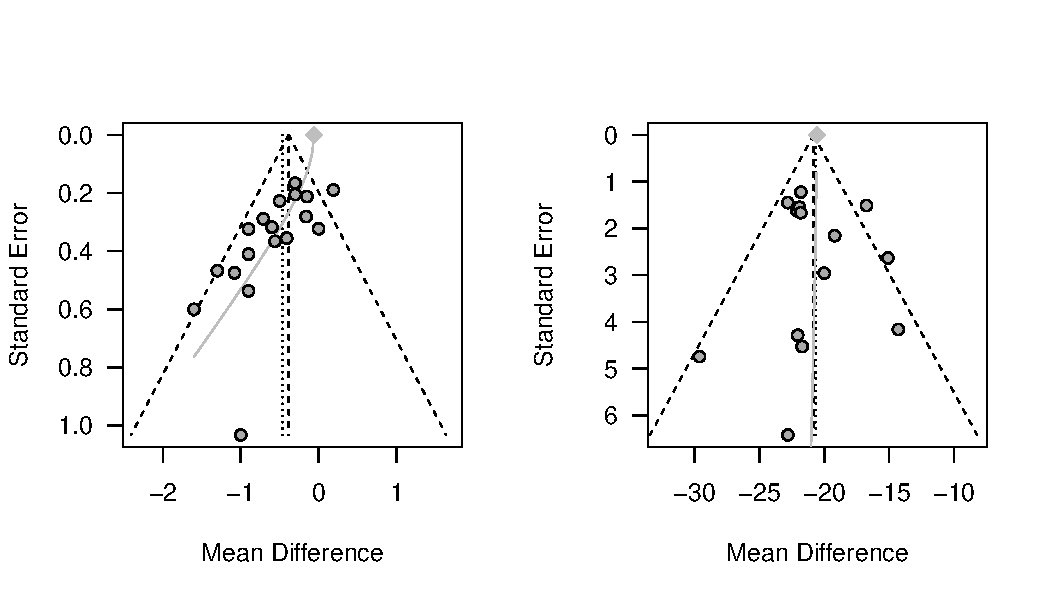
\includegraphics[width=\maxwidth]{figure/unnamed-chunk-9-1} 
\begin{kframe}\begin{verbatim}
## 
## 	Linear regression test of funnel plot asymmetry (methods of
## 	moment)
## 
## data:  meta.nexample
## t = -0.030699, df = 12, p-value = 0.976
## alternative hypothesis: asymmetry in funnel plot
## sample estimates:
##         bias      se.bias        slope 
##  -0.02266344   0.73825654 -20.60252776
\end{verbatim}
\end{kframe}
\end{knitrout}

\end{frame}



\begin{frame}{Regression based Tests}
Adjustments for binary outcomes:
\begin{itemize}
\item \citet{Peters} :$x_{i}$ = inverse of total sample size, $\textrm{variance}_{i}$ as weight.
\item \citet{Harbord} :$x:{i}$ = score of the log-likelihood of a proportion, $\textrm{variance}_{i}$ as weight.
\item \citet{Rucker} :Use arcsine variance stabilizing transformation for variances and effects, do e.g. Egger's test.
\end{itemize}
\end{frame}


\begin{frame}{Rank based tests}
\citet{begg.ties}
Let $y_{i}$ the standardized effect size of a study $i$, $v_{i}$ it's variance and $n$ the number of studies

$u$ the number of pairs $(y_{i}, v_{i})$ ranked in the same order, $l$
the number of pairs in the opposite order

$Z = (u - l)/\sqrt{n(n-1)(2n + 5)/18}$ \\ can be used as a test statistic (based on Kendall's Tau)
\end{frame}

\begin{frame}{Rank based tests}
\citet{Schwarzer}
Let $e_{t}$ the number of events in the treatment group

Given constant log odds ratio, $E_{t}$ follows a hypergeometric distribution.

$\mathbb{E}(E_{t})$ and the variance can be estimated and used as in 
\citet{begg.ties}
\end{frame}


\begin{frame}{Test Results}
Application of tests if:
\begin{itemize}
\item $n \geq 10$
\item at least one statistically significant effect in a study
\item $\frac{\sigma_{\textrm{max}}}{\sigma_{\textrm{min}}} > 4$
\item $I^2 < 0.5$
\end{itemize}

From 5338 with $n \geq 10$, 1602 remain.
\end{frame}

% \begin{frame}[fragile]{Test Results: Significance}
% 
% <<echo = FALSE, fig.height = 4>>=
% grid.arrange(p.bin, p.cont, ncol = 2)
% @
% \end{frame}

\begin{frame}[fragile]{Continuous Outcome Test Results}
$p$-values distribution:

\begin{knitrout}
\definecolor{shadecolor}{rgb}{0.969, 0.969, 0.969}\color{fgcolor}
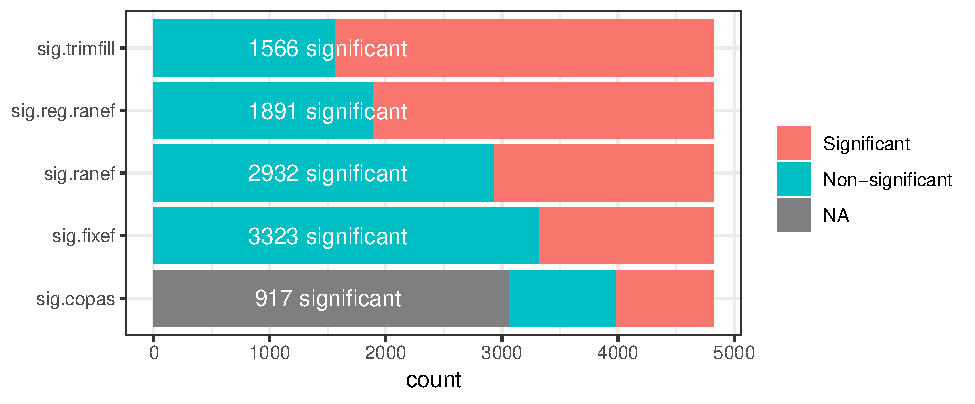
\includegraphics[width=\maxwidth]{figure/unnamed-chunk-10-1} 

\end{knitrout}
\end{frame}

\begin{frame}[fragile]{Binary Outcome Test Results}
$p$-values distribution:

\begin{knitrout}
\definecolor{shadecolor}{rgb}{0.969, 0.969, 0.969}\color{fgcolor}
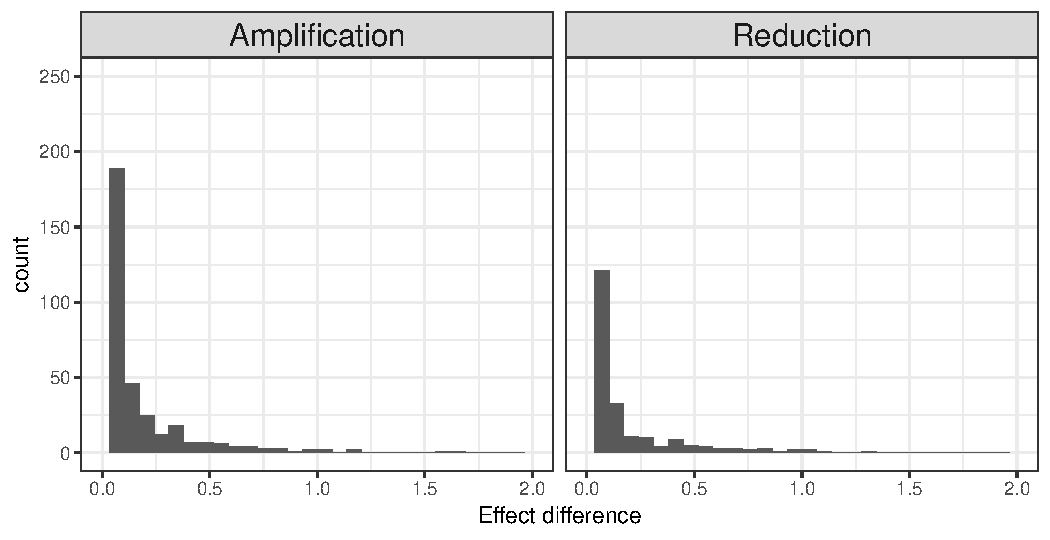
\includegraphics[width=\maxwidth]{figure/unnamed-chunk-11-1} 

\end{knitrout}
\end{frame}

\begin{frame}[fragile]{Agreement in significance}
Number of significant test results per meta-analysis:

\begin{knitrout}
\definecolor{shadecolor}{rgb}{0.969, 0.969, 0.969}\color{fgcolor}
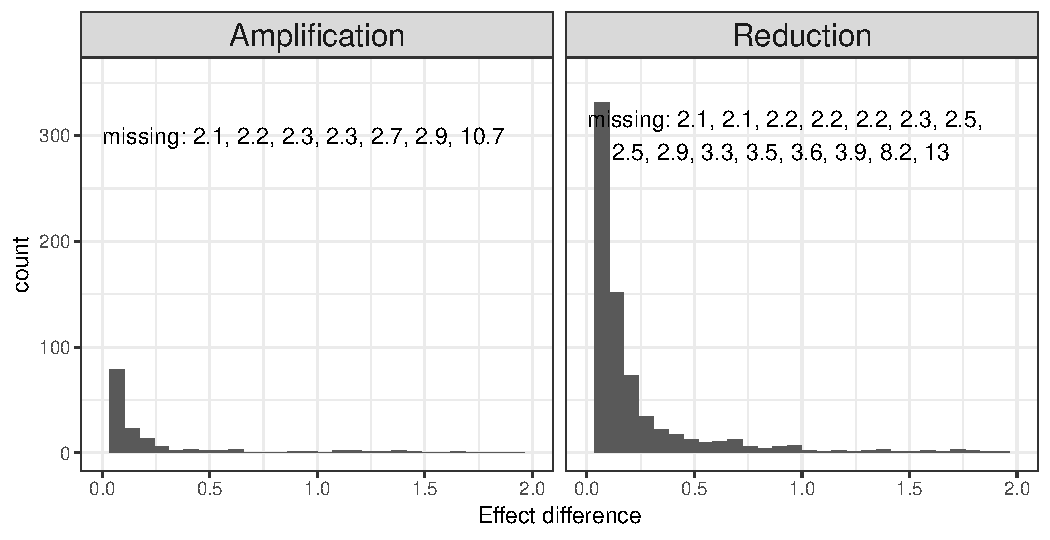
\includegraphics[width=\maxwidth]{figure/unnamed-chunk-12-1} 

\end{knitrout}
\end{frame}

\begin{frame}{Small Study Effect Adjustment}
Three methods:
\begin{itemize}
\item Regression
\item Copas selection model
\item Trim-and-fill
\end{itemize}
\end{frame}

\begin{frame}{Adjustment by regression}
Similar to the tests, but with unnormalized effect $y_{i}$:

\begin{align}
y_{i} = \beta_{0} + \beta_{1}x_{i}
\end{align}

$\beta_{0}$	 corresponds to $y_{i}$ with $x_{i} = 0$
\end{frame}

\begin{frame}[fragile]{Adjustment by regression}
Linear regression method:

\begin{knitrout}
\definecolor{shadecolor}{rgb}{0.969, 0.969, 0.969}\color{fgcolor}
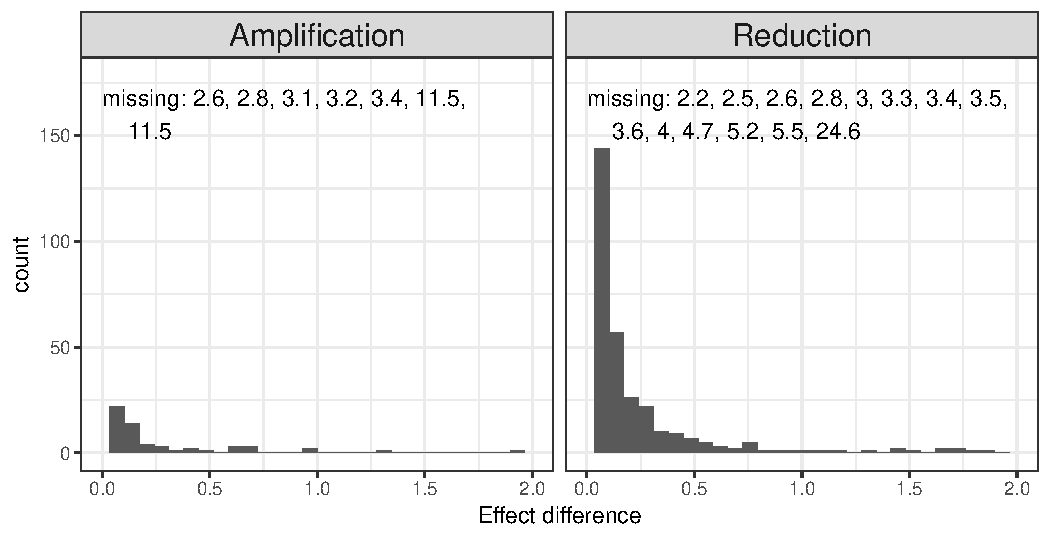
\includegraphics[width=\maxwidth]{figure/unnamed-chunk-13-1} 

\end{knitrout}
\end{frame}

\begin{frame}[fragile]{Shrinkage Regression}
Extended random effects model:

\vspace{-4mm}
\begin{align}
y_{i} = \beta_{0} + \beta_{1}(\sqrt{v_{i} + \tau^2}) + \epsilon_{i}(\sqrt{s_{i} + \tau^2}),  
\epsilon_{i} \stackrel{\textrm{iid}}{\sim} N(0,1) \nonumber
\end{align}

\vspace{-8mm}
\begin{align}
\mathbb{E}(y_{i}) \rightarrow \beta_{0} + \beta_{1}\tau \textrm{ if } \sqrt{v_{i}} \rightarrow 0 \nonumber
\end{align}

$\beta_{0}, \beta_{1}$ and $\tau$ can be estimated e.g. by ML and REML.
\end{frame}

\begin{frame}[fragile]{Shrinkage Regression}
shrinking the within study variance:

\vspace{-4mm}
\begin{align}
y_{i} &= \beta_{0}^\star + \beta_{1}^\star(\sqrt{v_{i}/M + \tau^2}) + \epsilon_{i}(\sqrt{s_{i}/M + \tau^2}) \nonumber
\end{align}

Letting $M \rightarrow \infty$ and substituting for all parameters and the observed residual

\vspace{-8mm}
\begin{align}
y_{\infty,i} &= \beta_{0}^\star + \sqrt{\frac{\tau^2}{v_{i} + \tau^2}}(y_{i} - \beta_{0}^\star)
\end{align}

\end{frame}

\begin{frame}[fragile]{Shrinkage Regression}
Three different treatment effect estimates:

\begin{align}
y_{\infty,i} &= \beta_{0}^\star + \sqrt{\frac{\tau^2}{v_{i} + \tau^2}}(y_{i} - \beta_{0}^\star)
\end{align}


\end{frame}




\begin{frame}{References}
  \small
  \bibliographystyle{apalike}
\bibliography{illustration}
\end{frame}



%\appendix
%% Possible backup slides...

%% chapter division is accomplished with:
%% \part{Appendix}

\end{document}
